\section{Figures and Tables \label{sec:figandtab}}

In Figure \ref{fig:selfie1} we can see a selfie taken by a macaque.
\begin{figure}[ht]
	\begin{center}
	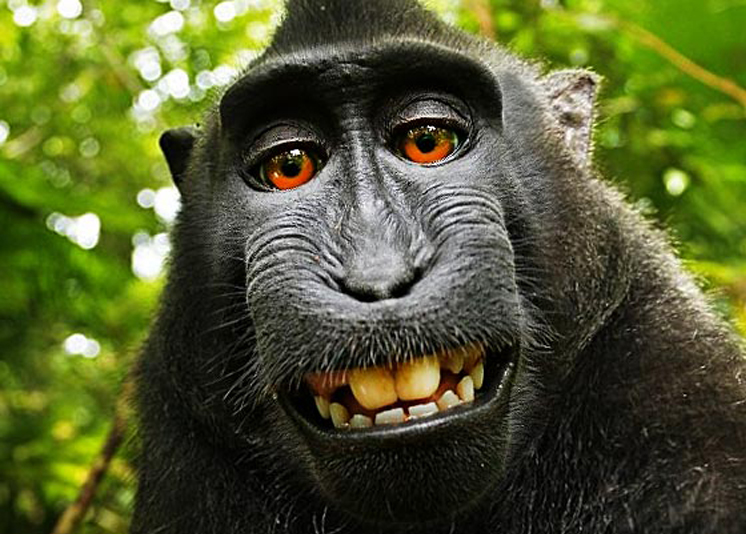
\includegraphics[width=0.5\textwidth]{./figures/selfie_monkey.jpg}
	\caption[Monkey selfie]{This picture is not copyrighted}
	\label{fig:selfie1}
	\end{center}
\end{figure}

Blandit incorrupte quaerendum in quo, nibh impedit id vis, vel no nullam semper audiam. Ei populo graeci consulatu mei, has ea stet modus phaedrum. Inani oblique ne has, duo et veritus detraxit. Tota ludus oratio ea mel, offendit persequeris ei vim. Eos dicat oratio partem ut, id cum ignota senserit intellegat. Sit inani ubique graecis ad, quando graecis liberavisse et cum, dicit option eruditi at duo. Homero salutatus suscipiantur eum id, tamquam voluptaria expetendis ad sed, nobis feugiat similique usu ex.

And now, Table \ref{tab:apvalues} shows some parameter for the Aliev-Panfilov model.
\begin{table}[H]
	\begin{center}
	\caption[Parameters Aliev-Panfilov]{Parameter values considered for the Aliev-Panfilov model of ionic current{\color{red}.}}
	\begin{tabular}{@{}c  c  c  c  c  c  c@{}}\toprule
	$\alpha$	&	$c_1$	&	$c_2$	&	$\mu_{1}$		&	$\mu_2$		&	$b$	&	$\gamma$\\ \midrule
	0.05	&	52	&	8	&	0.1	&	0.3	&	0.25	&	0.002 \\ \bottomrule
	\end{tabular}
	\label{tab:apvalues}
	\end{center}
\end{table}

There are 12 figures in order to show that the List of Figures works fine.

\section{Equations \label{sec:eq}}
Finally, an equation
\begin{equation}
x^2 + 1 = 0
\label{eq:basiceq}
\end{equation}

We can notice that $x=\pm i$ are the solutions of Equation \eqref{eq:basiceq}.